\chapter{cyk测试章节}

本章主要介绍仿真环境的搭建

\section{仿真环境搭建}

公式:
\begin{equation}
	a^2=b^2+c^2+d^2
\end{equation}

% Listing~\ref{lst:}

\begin{equation}
	OK
\end{equation}

\begin{figure}[htb]
	\centering 
	% 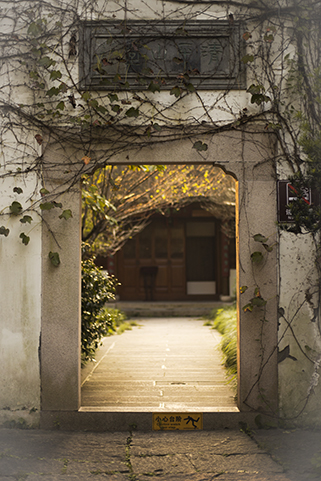
\includegraphics[width=\textwidth]{./Pictures/test.jpg} 
	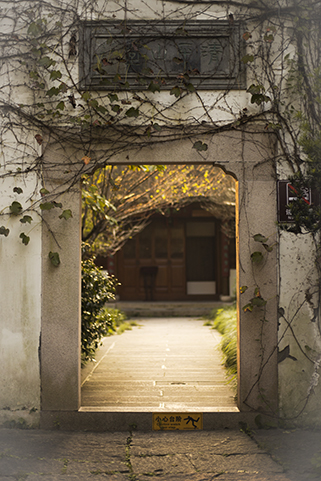
\includegraphics[scale=1.0]{./Pictures/test.jpg} 
	\caption{ljzst} 
\end{figure}

\begin{figure}[htb]
	\centering 
	% 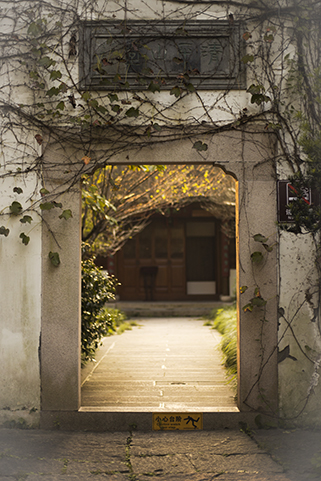
\includegraphics[width=\textwidth]{./Pictures/test.jpg} 
	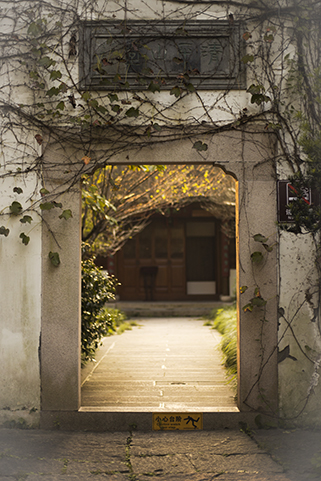
\includegraphics[scale=1.0]{./Pictures/test.jpg} 
	\caption{another way} 
\end{figure}

\begin{figure}[htb]
	\subfigure[img1]{ 
		\begin{minipage}[b]{0.5\textwidth} 
		\centering
		% \label{fig:SubFigure1} %% label for second subfigure 
		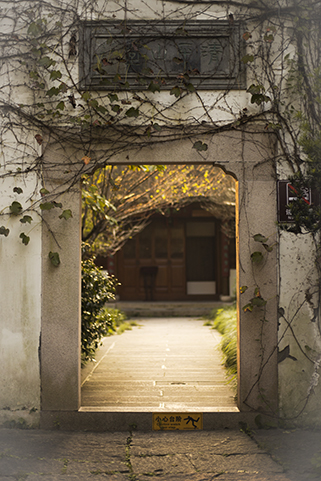
\includegraphics[scale=1.0]{./Pictures/test.jpg} 
		\end{minipage}}
	\subfigure[img2]{ 
		\begin{minipage}[b]{0.5\textwidth} 
		\centering
		% \label{fig:SubFigure1} %% label for second subfigure 
		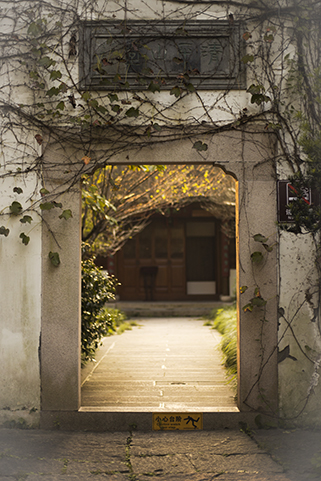
\includegraphics[scale=1.0]{./Pictures/test.jpg} 
		\end{minipage}}
	\caption{img all}
\end{figure}

{
\begin{table}[htb]
	\zihao{5}
	\caption{standard table} 
	% \label{Tabkeyword}
	\centering 
	\begin{tabular}[t]{
		|c|l|r|p{4cm}|} 
		\hline
		center & left & right & 靠左,并宽4cm\\ 
		\hline
		Center & Left & Right & Width=4cm\\ 
		\hline
	\end{tabular}
\end{table}
}

{
\begin{table}[htp]
	\zihao{5}
	\caption{复杂表格示例}
	% \label{TabComplex}
	\centering
	\begin{tabular}[t]{|c|c|c|c|c|}
		\hline
		\multicolumn{2}{|c|}{我占了两列} & 第3列 & 第4列 & 第5列\\
		\hline
		\multirow{2}*{我占了两行} & 第二行第2列 & 第二行第3列 & \multicolumn{2}{|c|}{\multirow{2}*{我占了两行又两列}}\\
		\cline{2-3}
		& 第三行第2列 & 第三行第3列 & \multicolumn{2}{|c|}{} \\
		\hline
	\end{tabular}
\end{table}
}



\section{OpenGL}

\subsection{投影变换}